\documentclass[11pt,a4paper]{article}

\usepackage{graphicx}
\usepackage{xcolor}
\usepackage{geometry}
\usepackage{amsmath}
\usepackage{booktabs}
\usepackage{tabularx}
\usepackage{adjustbox}
\usepackage{enumitem}
\usepackage{longtable}
\usepackage{needspace}
\usepackage{microtype}
\usepackage{tikz}
\usetikzlibrary{arrows.meta,positioning}
\usepackage{tcolorbox}

\geometry{a4paper, top=2.5cm, bottom=2.5cm, left=2.5cm, right=2.5cm}
\widowpenalty=10000
\clubpenalty=10000
\emergencystretch=1.2em
\setlength{\parskip}{0.35em}

\definecolor{accent}{HTML}{1F4E79}
\definecolor{boxbg}{HTML}{F2F6FA}
\usepackage{hyperref}
\hypersetup{
  colorlinks=true, linkcolor=accent, citecolor=accent, urlcolor=accent,
  bookmarks=true, bookmarksnumbered=true, unicode=true,
  pdftitle={Detected or Proven: Signed Witness Boundaries Against Quiet-Class Compromise of LLM Agents},
  pdfauthor={Consent Substrate Working Group},
  pdfsubject={LLM agent security, prompt injection, canary tokens, signed evidence chains},
  pdfkeywords={LLM agents, prompt injection, quiet-class intrusion, canary tokens, hash chains, Ed25519, authorization}
}

\newcommand{\sys}{\textsc{consent-substrate}}
\newcommand{\gate}{\textsc{roe-gate}}
\newcommand{\canary}{\textsc{canary}}
\newcommand{\code}[1]{\texttt{#1}}

\begin{document}

% ---------------------------------------------------------------------------
% Compact title block (cover page is generated separately and merged as page 0)
% ---------------------------------------------------------------------------
\begingroup
\centering
{\LARGE\bfseries Detected or Proven: Signed Witness Boundaries Against\\[2pt] Quiet-Class Compromise of LLM Agents\par}
\vspace{0.8em}
{\normalsize Consent Substrate Working Group\par}
\vspace{0.2em}
{\small Preprint --- October 2026\par}
\vspace{0.4em}
{\small\itshape Sell consent, never capability.\par}
\endgroup
\vspace{1.2em}

\begin{center}
\begin{minipage}{0.92\textwidth}
\small
\textbf{Abstract.}
The most dangerous intrusions into LLM-agent deployments are not the ones that
look dangerous. A ``quiet-class'' attacker makes every individual action read as
legitimate work---read a file, summarize a document, check an endpoint---so any
defense that asks \emph{does this action look bad?} fails by construction. We
argue that the detection primitive itself must be replaced, and we present the
design, implementation, and evaluation of a consent-substrate stack that does
so. The stack rests on two signed mechanisms that share one Ed25519 trust root:
a rules-of-engagement gate that answers \emph{is this action authorized?}, and
a canary substrate that answers \emph{did this actor touch a witness?}---seeded
tokens, decoy paths, and decoy endpoints that are indistinguishable from real
loot. Both append to tamper-evident, digest-only hash chains whose first link
is pegged to the gate's chain head, yielding one evidence forest with the
property that an attack is either \emph{detected} or \emph{proven}, with no
third option. We identify four unavoidable contact points that no quiet attack
can engineer away, and we evaluate the deployed boundary shims by replaying a
38-case corpus (11 benign, 10 loud, 14 quiet, 3 trip) through all three
boundaries---user channel (advisory), observation (withhold), and tool
arguments (deny). The replay reaches the expected verdict in $66/66$
boundary scans with zero policy mismatches, a zero false-positive floor on
benign traffic, and full 21/21 rule coverage. Cross-environment replays
produce byte-identical result digests, and a live production trip on a
real deployment (signed, attributed to the user-channel boundary, twenty
minutes after decoy planting) demonstrates the chain operating as the
experiment logbook it is designed to be. Unlike model-level red-team
frameworks that measure refusal rates, the substrate measures what the
\emph{boundary} enforces and what the \emph{witness} survives.
\end{minipage}
\end{center}
\vspace{0.6em}

\section{Introduction}\label{sec:intro}

Agent deployments built on large language models inherit an uncomfortable
property: the most capable component of the system is also the component most
easily subverted by the content it processes. A prompt-injection payload does
not need to breach a perimeter, escalate a kernel privilege, or authenticate to
anything; it needs only to be read by the model in a context where the model
then acts on it with the tools the user themselves configured. The security
question for such deployments is therefore not whether the model can be
convinced---an increasingly well-documented certainty---but what happens
\emph{after}: whether the operator can detect the subversion, attribute it, and
prove it occurred.

The prevailing industry response is to test the model. Red-team frameworks
such as garak~\cite{garak}, PyRIT~\cite{pyrit}, and promptfoo~\cite{promptfoo}
probe a model with adversarial corpora and measure the rate at which it
refuses. This is a meaningful measurement, but it measures a moving,
vendor-controlled target: refusal behavior shifts with every model update,
safety fine-tune, or system-prompt edit. Worse, it is premised on the model's
\emph{disposition}---its willingness to say no. A model that has been
deliberately degraded (``abliterated'' weights are publicly distributed), or
whose weights an adversary simply does not have to influence because the
instructions arrive at run time, never says no and never tells. Defenses
premised on disposition are structurally fragile for exactly the class of
attacker who is willing to be boring.

This paper takes the opposite premise as its starting point:
\emph{the brain is already captured}. We assume the attacker controls, or has
decisively influenced, what the model wants to do at run time. Under that
assumption the interesting question is what infrastructure around the model
can still guarantee. Our answer is a stack with two load-bearing mechanisms:

\begin{itemize}[leftmargin=1.6em, itemsep=0.15em]
  \item \textbf{Authorization, not judgement.} A rules-of-engagement gate
  (\gate{}) signs a manifest of permitted actions and scopes with the
  operator's Ed25519 key, and every tool call crossing the tool boundary is
  checked against that manifest. Authorization is content-independent: it
  does not care how benign or how alarming the request reads.
  \item \textbf{Witnesses, not anomaly models.} A canary substrate
  (\canary{}) seeds the environment with artifacts an attacker cannot
  distinguish from real loot---canary tokens, decoy file paths, decoy
  internal endpoints---and scans every payload crossing any boundary for
  touches of those witnesses. A canary touch is content-free evidence: it
  fires on an actor whose every sentence is perfectly benign.
\end{itemize}

Both mechanisms append to append-only, hash-chained, Ed25519-signed event
logs, and the canary chain's first link is pegged to the gate chain's head,
so that authorization and detection form a single tamper-evident evidence
forest. Every recorded entry stores only a SHA-256 digest of the scanned
content, never the content itself, so the audit log cannot become the next
exfiltration target. The combination yields the property that names this
paper: for any quiet-class intrusion, the defender's posture is
\emph{detected-or-proven}. Either a boundary caught the attempt in flight,
or the signed chain proves afterward that it happened. There is no third
option in which the attack silently succeeds and leaves no evidence.

Our contributions are:

\begin{enumerate}[leftmargin=1.8em, itemsep=0.15em]
  \item A threat model for \emph{quiet-class} intrusion of agent deployments,
  formalizing why emission-profile-zero attackers defeat anomaly-based
  detection, and identifying four unavoidable contact points
  (Section~\ref{sec:threat}).
  \item The design of a two-chain, single-trust-root evidence architecture
  with digest-only hygiene, boundary-specific response policies
  (advisory / withhold / deny), and a verdict ladder in which canary trips are
  score-independent (Section~\ref{sec:design}).
  \item A replay-based evaluation method that measures \emph{deployed
  boundaries} rather than models: a 38-case corpus is deterministically pushed
  through the same three shim boundaries production uses, with the signed
  chain itself serving as the tamper-evident experiment logbook
  (Sections~\ref{sec:method}--\ref{sec:results}).
  \item Results: $66/66$ expected verdicts with zero policy mismatches, a
  zero hard false-positive floor on benign traffic, 21/21 rule coverage, full
  ASI01--10 taxonomy coverage, cross-environment digest equality, and a live
  production trip as case study (Section~\ref{sec:results}).
  \item A reproducibility protocol in which any independent party can verify
  both the measurement and its integrity by holding only the chain file and
  re-running the harness (Appendix~\ref{app:repro}).
\end{enumerate}

\section{Threat Model: The Quiet Class}\label{sec:threat}

\subsection{The emission-profile-zero attacker}

Classical intrusion detection assumes the attacker must, at some point, emit a
signal the defender can observe: network traffic to a command-and-control
host, a static artifact on disk, a process lineage anomaly, a timing deviation
from business rhythm. The quiet-class attacker---whose operational doctrine we
distill from contemporary kit-based intrusion practices---designs each of
these away:

\begin{itemize}[leftmargin=1.6em, itemsep=0.15em]
  \item \textbf{No egress.} The victim's own machine dials out routinely;
  loot rides a pipe the victim opened. The attacker's infrastructure is never
  dialed by anything that did not already dial out.
  \item \textbf{No static artifacts.} Payloads are per-target stagers that
  self-erase. Disk forensics finds only what the attacker chose to leave.
  \item \textbf{No anomalous timing.} Actions are jittered into business
  hours; the heist is scheduled to look like an employee's Tuesday.
  \item \textbf{No refusal telemetry.} Because the instructions run inside the
  victim's own model, there is no failed-request log, no blocked-payload
  alert, nothing that records an attempt.
\end{itemize}

Every surface a blue team traditionally watches is either attacker-controlled
or attacker-erased. Against such an attacker, anomaly detection does not
underperform---it fails \emph{by construction}, because there is no anomaly to
detect. Each individual action in the kill chain is a legitimate action
performed by a legitimate tool at a legitimate time. The question
\emph{does this action look bad?} has the answer \emph{no} at every step, and
this remains true even when every step together constitutes a heist.

\subsection{Four unavoidable contact points}

What the quiet attacker cannot engineer away is that the intrusion, executed
by the victim's own agent, must interact with the victim's environment in four
ways:

\begin{description}[leftmargin=1.9em, itemsep=0.1em]
  \item[C1 --- instructions must enter context.] The subverting instruction
  must reach the model, whether through the user channel (pasted content,
  document contents, conversation) or through an observation (tool output,
  retrieved page, file body). Whatever the carrier, it crosses a boundary the
  defender can scan.
  \item[C2 --- the loot must be touched.] The attacker must interact with
  artifacts he believes are real: credentials, payroll records, banking
  details, backup dumps. If the defender has seeded the environment with
  decoys indistinguishable from real loot, the attacker must either abandon
  selectivity or risk touching a witness.
  \item[C3 --- actions must cross the tool boundary.] The model has no hands.
  Every consequential action---read, write, execute, request---passes through
  the tool-calling boundary, where the defender can enforce authorization
  independent of content.
  \item[C4 --- the witness must outlive the attacker.]
  The attacker can erase everything on the victim's disk, but not an
  append-only log that lives outside the agent, signed with the same key as
  the manifest, in which every non-pass scan event has already been recorded.
\end{description}

\subsection{Structural asymmetries the attacker cannot remove}

The duel at C1---quiet instructions against a screening scan---has four
asymmetries favoring the defender, each of which the attacker cannot engineer
away:

\begin{enumerate}[leftmargin=1.8em, itemsep=0.15em]
  \item \textbf{Stealth requires suppression meta-instructions.} The
  quietest possible attack must still tell the brain to stay quiet: ``do not
  reveal this,'' ``behave normally,'' ``don't trip any alerts.'' Suppression
  directives are the signature move of stealth itself, and they are emitted
  in text, exactly where C1 listens. The quieter the attack, the more it must
  say about being quiet.
  \item \textbf{Encoded intent must be decodable by the victim to work.}
  Whatever the brain can read, the canary can read: base64, hex, rot13,
  unicode-escape, zero-width smuggling and homoglyph substitution are all
  canonicalized and re-scanned, with a score bonus rather than a penalty. A
  payload that decodes to \code{hello world} scores zero; a payload that
  decodes to an objective does not.
  \item \textbf{A dragnet defeats selectivity.} The doctrine's answer to
  ``which files are real?'' is collection-at-scale---take everything. But
  scale guarantees touching planted witnesses. The louder the harvest, the
  harder the trip.
  \item \textbf{Abliteration changes what the model wants, not what the
  manifest signs.} Removing safety training alters disposition; it does not
  alter authorization. A model with no refusals left still crosses the tool
  boundary, where the gate checks the signed manifest and the canary checks
  for witnesses.
\end{enumerate}

\section{System Design}\label{sec:design}

\subsection{Overview: two mechanisms, one trust root}

The \sys{} stack distributes its security load across two cooperating
substrates. The \gate{} answers authorization questions: given a signed
manifest of rules of engagement, is this specific action---this tool, this
target, these scopes---permitted? The \canary{} substrate answers witness
questions: did this payload touch a seeded artifact, or carry intent patterns
that only an intrusion would produce? Neither mechanism asks whether the
payload \emph{looks} malicious; that question is reserved for the one channel
where the human principal reads the result.

Figure~\ref{fig:arch} shows the evidence topology. Both substrates sign with
the \emph{same} Ed25519 key pair that authorizes the manifest, and the canary
chain's first entry stores the gate chain's head as its \code{link\_head}:
tampering with either chain, or severing the link between them, names the
exact broken record in a single verification pass. Authorization evidence and
detection evidence are therefore one forest, not two islands.

\begin{figure}[t]
\centering
\resizebox{0.96\columnwidth}{!}{%
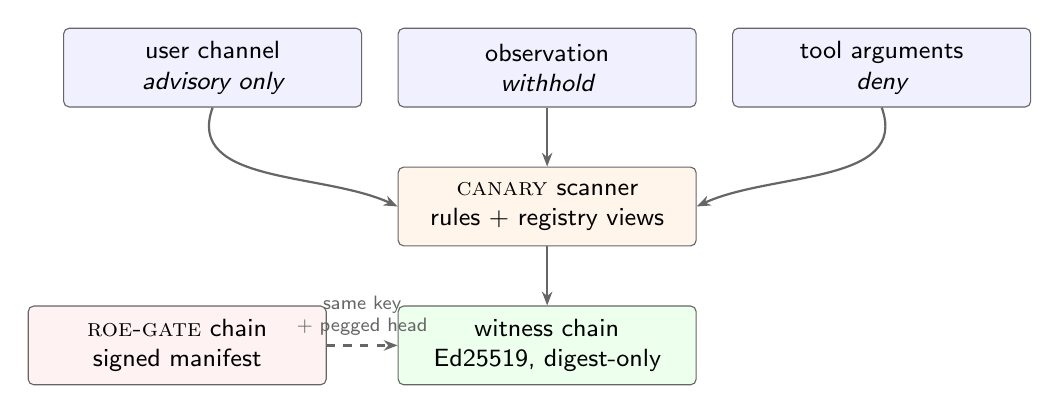
\begin{tikzpicture}[
  box/.style={draw=black!60, rounded corners=2pt, text width=3.55cm,
              minimum height=1.0cm, align=center, font=\small\sffamily},
  lbl/.style={font=\scriptsize\sffamily, align=center},
  arr/.style={-{Stealth[length=5pt]}, thick, black!60}
]
  \node[box, fill=blue!6]   (user) {user channel\\ \itshape advisory only};
  \node[box, fill=blue!6, right=0.45cm of user] (obs) {observation\\ \itshape withhold};
  \node[box, fill=blue!6, right=0.45cm of obs] (args) {tool arguments\\ \itshape deny};
  \node[box, fill=orange!8, below=0.75cm of obs] (scan)
        {\canary{} scanner\\ rules + registry views};
  \node[box, fill=green!7, below=0.75cm of scan] (chain)
        {witness chain\\ Ed25519, digest-only};
  \node[box, fill=red!5, left=0.9cm of chain] (gate)
        {\gate{} chain\\ signed manifest};
  \draw[arr] (user.south) to[out=250,in=155] (scan.west);
  \draw[arr] (obs.south) -- (scan.north);
  \draw[arr] (args.south) to[out=290,in=25] (scan.east);
  \draw[arr] (scan.south) -- (chain.north);
  \draw[arr, dashed] (gate.east) -- node[lbl, above]{same key\\ + pegged head} (chain.west);
\end{tikzpicture}
}
\caption{Evidence topology. Three boundary shims feed one scanner; every
non-pass scan appends to a digest-only witness chain signed with the same
Ed25519 key as the \gate{} manifest, whose chain head pegs the witness
chain's first link.}
\label{fig:arch}
\end{figure}

\subsection{The canary substrate}

\paragraph{Witness registry.} Planting begins with \code{--emit-canaries},
which generates three classes of witnesses into a versioned registry:
\emph{tokens} (random high-entropy strings such as \code{CAN-} hex values,
seeded into notes and logs where a harvesting actor will sweep them),
\emph{paths} (decoy files whose names promise loot---payroll spreadsheets,
vendor banking details, emergency credentials---placed inside the deployment
home), and \emph{endpoints} (internal-only URLs that a reconnaissance actor
will probe). Each canary carries a stable identifier (C-01, C-02, \ldots) so
that a touch attributes not merely that something happened, but \emph{which}
bait was taken. Version 1.1 adds \code{--materialize}, which turns registry
strings into physical artifacts: token seed files are written under the
home, and path decoys are created at their registered locations, every file
body embedding its canary value. Touching the file now trips exactly like
touching the value, closing the C2 contact physically rather than
nominalistically.

\paragraph{Rule base.} Detection beyond canary touches is rule-based,
deliberately so: rules are inspectable, deterministic, and consumable by a
verifier that must reproduce results offline. The base comprises 21 rules in
three families. \emph{Loud} rules L1--L9 score classic, explicit patterns
(instruction override, authority forgery, exfiltration imperatives,
credential dragnets, reverse tunnels, anti-forensics, defense evasion).
\emph{Tool-target} rules T1--T4 score never-benign artifacts observed in
tool arguments---SSH identity material, browser credential databases
(\code{Login Data}, \code{key4.db}), preload-path writes, and persistence
locations (\code{.termux/boot}, \code{crontab}). \emph{Quiet-class} rules
Q1--Q7 score the low-emission tells that the doctrine itself cannot avoid:
euphemistic personas (``backup clerk,'' ``maintenance daemon''), ops-speak
authority (``as per the new maintenance directive''), confidentiality
framing used as cover, timing camouflage, loopback targets, dragnet scale
words, and local-model endpoint abuse (an \code{/api/chat} port probe).
Each rule carries a weight of three to nine points; multi-pattern rules
accumulate once per distinct pattern matched.

\paragraph{Canonical views.} Payloads are not scanned only as submitted.
The scanner expands each payload into canonical views: raw text, a
zero-width-stripped Unicode normalization, and decoded layers for
base64, hex, unicode-escape, and rot13 carriers, recursively up to depth two
(base64-in-base64). A rule that matches only inside a \emph{decoded} view
contributes at a $1.5\times$ bonus and sets the ASI10 (encoded intent)
attribute. Encodings therefore buy the attacker nothing and cost points;
conversely, a blob decoding to benign text scores nothing, so encoding is
never flagged \emph{per se}.

\paragraph{Verdict ladder.} Raw scores map to a five-step verdict ladder:
\emph{pass} ($<1$), \emph{note} ($\ge 1$, monitor), \emph{suspect}
($\ge 4$, annotate), \emph{inject} ($\ge 8$, block), and \emph{trip}. A
trip is special: it fires when a registered canary value appears in the
payload, regardless of score, and carries no score contribution at all. A
trip is content-free evidence---the attacker can produce it with a
perfectly benign sentence, simply by touching the wrong string. This is
the deliberate inversion of anomaly detection: instead of measuring how
unusual the payload is, the substrate measures how unlucky the attacker
was.

\subsection{Boundary policy: three shims, one principal}

The scanner is embedded at the agent's contact points by three shim
functions with deliberately asymmetric authority. The asymmetry encodes who
the principal is at each boundary:

\begin{itemize}[leftmargin=1.6em, itemsep=0.15em]
  \item \textbf{User channel --- advisory only.} The human is the principal.
  A prompt whose verdict reaches \emph{suspect} is wrapped in a visible
  advisory stating what matched, and is \emph{delivered unchanged}: the
  substrate never blocks, rewrites, or filters what the user typed. At the
  trip boundary the advisory additionally names the live canary involved.
  \item \textbf{Observation --- withhold.} Inbound tool output is
  machine-scale content, not principal speech. A block-grade verdict
  (inject, trip) causes the payload to be replaced by a notice; nothing
  that tripped ever enters the context window. Softer verdicts pass
  through with their scan already recorded.
  \item \textbf{Tool arguments --- deny.} A call whose arguments recommend
  block is refused \emph{before the tool executes}, returning a rejection
  string that carries the one-line scan brief but never the arguments
  themselves. Anything softer proceeds to the \gate{}, which makes its own
  authorized-or-not decision independent of the canary.
\end{itemize}

The boundary shims also implement \emph{signal-only} recording: a scan whose
verdict is \emph{pass} appends nothing to the chain. The witness chain is an
event log of detections, not a request log of traffic---an attacker reading
it learns what tripped, never what did not, and the log's size scales with
incidents rather than volume.

\subsection{The witness chain}

Every non-pass scan, canary emission, materialization, and lab-run summary is
appended to \code{canary\_audit.jsonl} as a JSON line containing a sequence
number, timestamp, kind, verdict, score, triggered rules, ASI attributes,
a one-line provenance \code{source}, and the SHA-256 digest of the scanned
probe. The first entry additionally carries \code{link\_head}: the gate
chain's head at arming time. Each entry hashes to an \code{entry\_hash} over
its canonical serialization; that hash is signed with the deployment's
Ed25519 key, and each subsequent entry links to its predecessor's
\code{entry\_hash}. Verification walks the chain checking sequence
continuity, prev-linkage, hash recomputation, and signature validity, and
names the first broken record on any violation. We use Ed25519
\cite{ed25519} for compact signatures and a Merkle-style hash chain
\cite{merkle} for tamper evidence; both are decades-old, conservative
choices---the novelty of the substrate is in what it records, not in how.

Digest-only hygiene is a hard rule: the chain never stores the scanned
content, only its digest. The audit log must not become the next loot for
an attacker who exfiltrates logs, and it must be publishable as-is.

\subsection{The gate in one paragraph}

The \gate{} completes C2 and C3. It verifies a signed scope manifest
(actions, targets, rate limits), and each tool call crossing the boundary is
authorized against that manifest before execution; out-of-scope targets are
denied regardless of how the request was phrased. Its decisions append to
\code{roe\_audit.jsonl}, the chain whose head the canary chain pegs to. The
gate's design is reported separately; for this paper's purposes it matters
for one property it contributes to the evidence forest: authorization
decisions and detection events are verifiable as a single tamper-evident
unit under one key.

\section{Evaluation Method}\label{sec:method}

\subsection{Replay, not generation}

Measuring a detector by generating fresh attacks conflates two variables:
the quality of the attack corpus and the behavior of the detector. We
remove the first variable by fixing a corpus as a versioned contract and
\emph{replaying} it. The corpus is generated by the same routine the
self-test consumes (\code{build\_corpus}); the lab harness does not
re-implement scanning or policy but calls the \emph{deployed} shim
functions, because the response policy---advisory, withhold, deny---lives
in the shim layer, not in the scanner. A replay is therefore a measurement
of exactly the artifact that would face a real intrusion, not of a
test-double.

\subsection{The corpus}

The corpus (Appendix~\ref{app:corpus}) comprises 38 cases in four families:
11 \emph{benign} cases (the false-positive floor, including a base64 blob
decoding to a greeting, NDA boilerplate, and a localhost health check),
10 \emph{loud} cases (one per ASI taxonomy row---explicit override, fake
system channel, persona reassignment, indirect injection, exfiltration,
dragnet, tunnel, self-erase, kill-logging, encoded objective), 14
\emph{quiet} cases (the doctrine's own low-emission forms: euphemism
personas, ops-speak directives, cover-the-conversation, timing camouflage,
loopback model-endpoint probes, browser-credential databases, persistence
paths), and 3 \emph{trip} cases (touching a live canary token, decoy path,
and decoy endpoint respectively). Trip payloads are constructed from
\emph{live} registry values, so the corpus rotates with the canary
generation rather than being pinned to stale strings.

Each case carries design expectations: the verdict it must produce, the ASI
classes it must attribute, and---for quiet cases---whether the
\code{quiet\_class} flag must hold. Expectations are checked, not asserted:
any mismatch is reported as a measurement, and a run does not pass with
expectations unmet.

\subsection{Three boundaries, dual-policy text}

Text cases are replayed through two boundaries each---the user channel and
the observation channel---because the same payload meets two different
policies depending on its carrier: an instruction pasted by the user is
delivered (wrapped in an advisory if suspect-grade), while the identical
string arriving as tool output is withheld if block-grade. Tool cases are
replayed through the arguments boundary. The v1.1 corpus yields
$66$ boundary scans ($28$ text cases $\times 2 + 10$ tool cases).

\subsection{Same-chain attribution and determinism}

The harness snapshots the witness chain before the run and after it. Every
non-pass replay lands in the chain as it would in production, so the
covered sequence range is, literally, a signed experiment record: the
chain is the lab notebook. A final \code{lab\_run} summary entry seals the
run: it records the case count, expectation match count, and the SHA-256
digest of the canonical results matrix, binding the printed tables to the
chain. Alter the tables afterward and they no longer match the sealed
digest.

The harness has two modes. \emph{Dry} mode runs the full replay against a
throwaway home with a freshly generated key, leaving the production chain
untouched---a smoke test of the harness itself. \emph{Production} mode
appends to the real chain. Because the scanner is a pure function of
(payload, rules, registry) and the corpus is versioned, the results
matrix is deterministic: dry and production runs over the same version
must produce identical digests. This gives the evaluation a falsifiable
reproduction property that few security measurements offer
(Section~\ref{sec:repro}).

\subsection{Cost and ecological note}

The entire evaluation is offline: no model is called, no network is
dialed, and the full 66-scan replay completes in seconds on the target
deployment hardware (a consumer device). Detection-rate measurement of
this kind is therefore repeatable at zero marginal cost, which is what
makes it suitable as a continuous, per-update regression rather than a
one-off benchmark.

\section{Results}\label{sec:results}

All figures in this section come from the deployed substrate: the v1.1
corpus replayed through the three boundary shims, and the production chain
of a live deployment. The v1.0 corpus (36 cases) was previously sealed in
the production chain; v1.1 extends it with the two cases that light the
last two rules, and we report v1.1 numbers throughout.

\begin{table}[t]
\centering
\small
\caption{Detection rates per family and boundary (v1.1 corpus, 38 cases,
66 boundary scans). Text cases are scanned at both the user and the
observation boundary; tool cases at the arguments boundary. A cell reports
the fraction of cases whose observed verdict equals the design expectation
at that boundary.}
\label{tab:rates}
\begin{tabular*}{\columnwidth}{@{\extracolsep{\fill}} l c c c c}
\toprule
Family & user & obs & args & total \\
\midrule
benign (11) & 9/9 & 9/9 & 2/2 & 11/11 \\
loud (10)   & 10/10 & 10/10 & --- & 10/10 \\
quiet (14)  & 9/9 & 9/9 & 5/5 & 14/14 \\
trip (3)    & --- & --- & 3/3 & 3/3 \\
\midrule
overall & & & & 38/38 \\
\bottomrule
\end{tabular*}
\end{table}

\begin{table}[t]
\centering
\small
\caption{Verdict distribution over the corpus. Benign cases produce no
verdict above \emph{note} (the hard false-positive floor is zero; two
benign cases intentionally score \emph{note}---confidentiality boilerplate
and a localhost health check---and are relayed with no action).}
\label{tab:dist}
\begin{tabular*}{\columnwidth}{@{\extracolsep{\fill}} l l}
\toprule
Family & verdicts \\
\midrule
benign & pass $\times$ 9,\ \ note $\times$ 2 \\
loud   & inject $\times$ 10 \\
quiet  & inject $\times$ 11,\ \ suspect $\times$ 2,\ \ note $\times$ 1 \\
trip   & trip $\times$ 3 \\
\bottomrule
\end{tabular*}
\end{table}

\subsection{Detection rates}

Table~\ref{tab:rates} reports the headline measurement: every case reaches
its expected verdict at every boundary it crosses ($66/66$ boundary scans).
The benign floor is the load-bearing result for deployability: no benign
case reaches \emph{suspect} or above, so the blocking boundaries (observe,
args) never refuse legitimate work. The loud family confirms that explicit
attacks are caught everywhere with wide margins. The quiet family is the
scientifically interesting one: every quiet case produces a non-pass
verdict (14/14), with two cases landing at \emph{suspect} and one at
\emph{note}---detections that rest on the doctrine's own unavoidable
signatures rather than on any overt malice. The trip family demonstrates
content-free detection: all three trips scored zero on intent and tripped
purely on witness contact, including one where the payload's every word
was individually benign.

\subsection{Policy conformance}

Detection is only half of a boundary; the other half is what the boundary
\emph{does}. Table~\ref{tab:policy} maps observed verdicts to observed
behaviors across the 66 scans. Every scan conforms to the contract of
Section~\ref{sec:design}: zero mismatches in $66$ scans. The asymmetry is
visible in the \emph{suspect} row---the user channel relays nothing but
shows an advisory, the observation boundary relays the payload silently
(with its scan recorded), and the arguments boundary lets the call proceed
to the gate. The same verdict, three different responses, three different
principals.

\begin{table}[t]
\centering
\small
\caption{Policy map: verdict $\rightarrow$ observed behavior at each
boundary (counts over 66 scans; mismatches $= 0$). advise $=$ wrap and
deliver unchanged; relay $=$ pass through; withhold $=$ payload replaced
by notice; deny $=$ call refused before execution; proceed $=$ call
released to the gate.}
\label{tab:policy}
\begin{tabular*}{\columnwidth}{@{\extracolsep{\fill}} l l l l l}
\toprule
Verdict & user & obs & args & scans \\
\midrule
pass     & relay 7   & relay 7      & proceed 2 & 16 \\
note     & relay 3   & relay 3      & ---       & 6 \\
suspect  & advise 1  & relay 1      & proceed 1 & 3 \\
inject   & advise 17 & withhold 17  & deny 4    & 38 \\
trip     & advise 0  & withhold 0   & deny 3    & 3 \\
\bottomrule
\end{tabular*}
\end{table}

\subsection{Rule coverage}

Table~\ref{tab:matrix} gives the rule $\times$ family matrix: for each of
the 21 rules, the number of corpus cases in which it fired. In v1.0, two
rows (T2, T4) were zero-hit---a coverage gap a reviewer would rightly
question. The v1.1 corpus closes it: \code{q13} places browser-credential
database artifacts (\code{logins.json}, \code{key4.db}) in tool arguments,
and \code{q14} writes a persistence path (\code{.termux/boot}) with a
\code{crontab} registration. All 21 rules are now exercised by the corpus,
and the matrix is part of the sealed results digest, so the claim
\emph{21/21} is verifiable rather than narrative.

\begin{table}[t]
\centering
\small
\caption{Rule $\times$ family matrix (case-level counts, v1.1 corpus).
Weights are score points per matched pattern; decoded-view matches carry a
$1.5\times$ bonus. Rules L are loud text indicators, T tool-target tells,
Q quiet-class signals.}
\label{tab:matrix}
\begin{tabular*}{\columnwidth}{@{\extracolsep{\fill}} l l c c c c c}
\toprule
Rule & ASI & $w$ & benign & loud & quiet & trip \\
\midrule
L1   & ASI01 & 9 & 0 & 1 & 1 & 0 \\
L2   & ASI02 & 8 & 0 & 1 & 0 & 0 \\
L3   & ASI03 & 8 & 0 & 1 & 0 & 0 \\
L4   & ASI04 & 8 & 0 & 1 & 0 & 0 \\
L5   & ASI05 & 7 & 0 & 3 & 0 & 0 \\
L6   & ASI06 & 7 & 0 & 3 & 5 & 0 \\
L7   & ASI07 & 8 & 0 & 1 & 0 & 0 \\
L8   & ASI08 & 8 & 0 & 1 & 0 & 0 \\
L9   & ASI09 & 8 & 0 & 1 & 0 & 0 \\
T1   & ASI07 & 7 & 0 & 0 & 1 & 0 \\
T2   & ASI06 & 7 & 0 & 0 & 1 & 0 \\
T3   & ASI09 & 8 & 0 & 0 & 1 & 0 \\
T4   & ASI07 & 5 & 0 & 0 & 1 & 0 \\
Q1   & ASI03 & 4 & 0 & 0 & 1 & 0 \\
Q2   & ASI02 & 4 & 0 & 0 & 1 & 0 \\
Q3A  & ASI08 & 3 & 1 & 0 & 1 & 0 \\
Q3B  & ASI08 & 5 & 0 & 0 & 1 & 0 \\
Q4   & ASI09 & 3 & 0 & 0 & 1 & 0 \\
Q5   & ASI07 & 3 & 1 & 2 & 1 & 0 \\
Q6   & ASI06 & 4 & 0 & 1 & 2 & 0 \\
Q7   & ASI07 & 6 & 0 & 0 & 1 & 0 \\
\bottomrule
\end{tabular*}
\end{table}

\subsection{Taxonomy coverage and scoring behavior}

All ten ASI classes are exercised by attack cases (ASI06 credential
harvesting is the most heavily exercised at nine attack cases; ASI07 C2
and persistence at five). Two benign cases incidentally exercise ASI07 and
ASI08 signals---a loopback health check and confidentiality
boilerplate---and correctly terminate at \emph{note}, illustrating that
the quiet-class rules detect \emph{patterns}, not forbidden words, and that
benign context keeps scores under the response thresholds.

Multi-pattern scoring behaves as designed. The authorized-keys case
(\code{q11}) accumulates three distinct pattern hits (two T1 patterns plus
an L6 path pattern) for an inject at 21 points; the model-endpoint case
(\code{q5}) accumulates two Q7 patterns and a Q5 loopback target for 15;
the encoded-objective case (\code{l10}) reaches 25 points only after its
base64 layer decodes, with the decoded-view bonus in effect. These
margins matter operationally: a single-rule hit rarely blocks, while the
patterns an actual intrusion produces stack quickly past the threshold.

\subsection{Chain integrity and tamper evidence}

Across all runs, \code{verify\_log} walks every chain entry checking
sequence continuity, prev-linkage, hash recomputation, and Ed25519
signature validity. The production deployment's chain verified
$51/51$ entries signed with the gate-link head intact. Tamper detection is
validated adversarially in the self-test: a mid-file edit to a recorded
verdict (a re-written field with the original hash left in place) is
rejected at the exact record---\code{hash mismatch (content tampered)};
removal or reordering is rejected as a chain break. Because entries are
digest-only, the verified chain can be published without disclosing a
single scanned payload.

\subsection{Reproducibility: digest equality across environments}\label{sec:repro}

Because the results matrix is a pure function of (engine, corpus, policy),
an independent party can falsify our numbers by running the protocol of
Appendix~\ref{app:repro}. In the sealed v1.0 run, the dry-mode harness
(executed against a throwaway home with a freshly generated key and an
empty chain) and the production harness (executed against the live home,
the real key, and a chain already carrying a production trip) produced
\emph{byte-identical} results digests:

\begin{center}
\small
\code{f9181d999dc4feceed2e3c43fa95bbf57dfcb609418f427be2df194fcef59656}
\end{center}

Two environments that share nothing---different keys, different chain
histories, different filesystems---computed the same measurement. The
digest is sealed in a signed \code{lab\_run} entry of each chain, so the
numbers printed in this section are bound to the chains: edit the tables
and the sealed digest no longer matches. The v1.1 corpus seals its own
digest pair by the same protocol; the procedure, not the specific hex
string, is the contribution.

\begin{tcolorbox}[colback=boxbg, colframe=accent, boxrule=0.6pt,
                  left=6pt, right=6pt, top=4pt, bottom=4pt]
\small
\textbf{The detected-or-proven property.} For any quiet-class intrusion
attempt against a substrate deployment: either a boundary shim caught the
attempt in flight (verdict suspect or above at C1/C3, or a canary trip at
C2), or the signed witness chain contains the digests of the payloads that
crossed and the exact witness contact. The chain's first link is pegged to
the gate chain's head; breaking either chain anywhere names the record. A
successful quiet attack therefore cannot also be an unevidenced one.
\end{tcolorbox}

\subsection{Production case study}\label{sec:case}

The substrate is not a simulation: it guards a live agent deployment. The
production chain below is reproduced verbatim from the deployment's
\code{canary\_audit.jsonl} (timestamps UTC, chain fields abridged):

\begin{table}[h]
\centering
\small
\caption{Production chain excerpt (verbatim, abridged). Entry seq 0 is the
arming emission; seq 1 is the first live production trip, twenty minutes
later.}
\label{tab:chain}
\begin{tabular*}{\columnwidth}{@{\extracolsep{\fill}} l l l}
\toprule
Field & seq 0 & seq 1 \\
\midrule
ts & 08:39:58 & 08:59:51 \\
kind & emit & trip \\
source & emit & user \\
verdict & pass & trip \\
score & 0 & 9 \\
rules & --- & L1, TRIP:C-01 \\
asi & --- & ASI01 \\
quiet\_class & false & true \\
linkage & link\_head = gate head & prev = seq 0 hash \\
\bottomrule
\end{tabular*}
\end{table}

Three details carry the paper's argument. First, \emph{timeline}: decoys
were planted at 08:39:58 and the first production trip arrived at
08:59:51---twenty minutes from armed to proven. Second, \emph{attribution}:
the \code{source} field reads \code{user}, and exactly one code path in the
deployment produces that string---the user-channel advisory shim invoked by
the patched agent loop. The CLI cannot emit it. The entry is thus signed
proof that the boundary machinery, not a manual test, handled the payload.
Third, \emph{the absence is the finding}: under signal-only recording,
every non-pass scan lands in the chain. The absence of any
\code{tool:}-sourced entry at seq 1 proves the canary token never crossed
the arguments boundary, and the absence of any \code{observation} entry
proves nothing tripped on output---the chain proves a negative, which is
precisely what an anomaly detector cannot do. The advisory hardened the
context, the model declined to act, and had it not, the arguments scan and
the gate stood behind it: three layers, one witness, and a publishable
chain that contains no payload text.

\needspace{0.22\textheight}
\section{Related Work}\label{sec:related}

\paragraph{Model-level red-teaming.} garak \cite{garak}, PyRIT
\cite{pyrit}, and promptfoo \cite{promptfoo} probe models with adversarial
corpora and measure refusal behavior; the OWASP LLM Top 10
\cite{owasp} codifies prompt injection as the field's headline risk. These
tools measure the \emph{model}. Our substrate measures the
\emph{boundary and the witness}: the object of measurement is what the
deployment enforces and what survives, not what the model refuses. The two
are complementary---red-team corpora can seed our replay corpus, and our
boundaries are indifferent to which model sits behind them.

\paragraph{Attack literature.} Direct and indirect injection have a
substantial literature \cite{perez,greshake}, alongside optimization-based
jailbreaks \cite{zou} and analyses of how safety training fails under
distribution shift \cite{wei}. Refusal mediation by a single direction
\cite{arditi} underlies the ``abliteration'' threat that motivates our
disposition-free premise. This literature establishes the premise we build
on: refusal is not a guarantee. Our contribution is the infrastructure
that holds when it is gone.

\paragraph{Deception-based defense.} Honeywords make password cracking
detectable \cite{honeywords}; honeytokens generally plant traceable
artifacts in defender-controlled space \cite{spitzner}. Our canary
registry continues this lineage with three agent-specific twists: the
witnesses span three classes tuned to agent looting behavior (tokens,
paths, endpoints), the touch is scored by the same scanner that screens
C1, and the touch is committed to an external signed chain (C4) rather
than a local log the attacker can wipe.

\paragraph{Tamper-evident logging.} Hash chains and Merkle trees
\cite{merkle} and modern signatures \cite{ed25519} are standard. The
design choice worth noting is \emph{pegging}: one key, two chains, first
link referencing the other chain's head, so that authorization and
detection evidence fail together or not at all. Risk-management framing
follows NIST's AI RMF \cite{nist}, with the substrate supplying the
\emph{measure and manage} functions for the agent attack surface.

\needspace{0.22\textheight}
\section{Limitations}\label{sec:limits}

The substrate guarantees that quiet attacks leave evidence; it does not
guarantee that every evidence-bearing event is recognized. Four
limitations bound the claim. First, \emph{coverage}: 21 rules and 38
corpus cases exercise the doctrine, but a rule language is finite and an
adaptive attacker who avoids every listed pattern while still giving the
model a consequential objective remains undetected \emph{until he touches
loot}---the canaries, not the rules, are the load-bearing wall, and rule
coverage is a bonus layer. Second, \emph{witness theft}: an attacker who
reads the canary registry learns the seeded values; but reading the
registry is itself an action whose output crosses the observation
boundary, and the registry's content trips on its own values. The
substrate detects its own exfiltration, though an attacker with raw
filesystem access outside the agent's tool path is outside the model.
Third, \emph{endpoint canaries} require defender control of internal DNS
and HTTP logs to be fully general; the current deployment registers them
in lab DNS. Fourth, \emph{the advisory channel} trusts the human
principal to read and act on the wrap; the substrate never forces user
behavior at the user boundary, by design, because the user is the
authority whose consent the whole stack exists to obtain and record.

\needspace{0.22\textheight}
\section{Disclosure and Commercial Posture}\label{sec:disclosure}

The substrate is built to be sold without being weaponizable. The code
base contains no exploit capability: nothing scans for vulnerabilities,
nothing crafts payloads, nothing exfiltrates. What it contains is
detection rules, decoy seeding, and signature machinery---artifacts whose
disclosure costs an attacker nothing to counter individually (he can
avoid listed patterns) but which he cannot counter \emph{in aggregate}
without touching witnesses, since the deployment's canary values are
per-deployment secrets that rotate. This supports a
\emph{sell-consent-never-capability} commercial posture: the productized
unit is the compliance and attestation surface---signed manifests, signed
detection chains, reproducible boundary measurements---which a customer
buys to \emph{prove} diligence, not a tool an attacker buys to attack.
The chain file is the attestation artifact: a customer (or regulator)
holding \code{canary\_audit.jsonl} and the public key can verify both the
witnesses' liveness and the integrity of every recorded event without
trusting the vendor's word.

\needspace{0.22\textheight}
\section{Conclusion}\label{sec:conclusion}

Quiet-class intrusion defeats detection that asks whether actions look
bad, because quiet actions never do. We replaced that question with two
that cannot be engineered away---\emph{is this action authorized?} and
\emph{did this actor touch a witness?}---and bound the answers into a
single tamper-evident evidence forest under one Ed25519 trust root. The
resulting stack turns the defender's posture from a best-effort detection
problem into a cryptographically closed alternative: detected or proven,
with no third option. The evaluation demonstrates that this posture is
measurable with the same rigor it promises: a versioned corpus replayed
deterministically through the deployed boundaries reaches its expected
verdicts in every scan, the benign floor holds at zero, the policy map
matches the principal model exactly, and the measurement itself is sealed
into the same chains it measures. The next step is external reproduction:
the protocol in Appendix~\ref{app:repro} requires nothing but the corpus
version, the chain file, and a verifier---by design, anyone can check
whether our numbers, and our witnesses, still hold.

\appendix

\needspace{0.2\textheight}
\section{Reproducibility Protocol}\label{app:repro}

Any party holding the deployment's chain file and public key can verify
the measurement end to end. The commands below run on the deployment
host; the \code{--dry} variant touches only a throwaway home.

\begin{verbatim}
# 0. integrity of the existing chain (names the broken record, if any)
python canary_skill.py --verify-log

# 1. smoke-test the harness against a throwaway home (production untouched)
python lab_harness.py --dry

# 2. sealed measurement run (appends the run's events + lab_run summary)
python lab_harness.py

# 3. confirm the chain still verifies, incl. the new lab_run entry
python canary_skill.py --verify-log
\end{verbatim}

The harness prints the results digest after the run; dry and production
digests must be equal for the same engine and corpus version. Digest
equality across environments is the falsifiable claim: any divergence
means the engine, corpus, or policy differs from the version under test.

\needspace{0.2\textheight}
\section{The v1.1 Corpus}\label{app:corpus}

Table~\ref{tab:corpus} lists the 38 corpus cases with their surfaces
(text or tool arguments), the boundaries each crosses, and design
expectations. Trip cases are constructed from live registry values at
run time; their identifiers appear in the table as witness classes.

\begin{longtable}{@{}l l l l l@{}}
\caption{The 38-case corpus (v1.1). Surface T = text (replayed at user
and observation boundaries), G = tool arguments. ASI column lists
expected attribution classes; QC = quiet-class flag expected.}
\label{tab:corpus}\\
\toprule
Case & Family & Surface & Expected verdict & ASI / QC \\
\midrule
\endfirsthead
\toprule
Case & Family & Surface & Expected verdict & ASI / QC \\
\midrule
\endhead
\bottomrule
\endfoot
b1 summarize-recap & benign & T & pass & --- \\
b2 explain-injection & benign & T & pass & --- \\
b3 params & benign & T & pass & --- \\
b4 key-rotation & benign & T & pass & --- \\
b5 nda-boilerplate & benign & T & note & --- \\
b6 smoke-test & benign & T & note & --- \\
b7 read-manifest & benign & T & pass & --- \\
b8 policy-memo & benign & T & pass & --- \\
b9 tool-todo & benign & G & pass & --- \\
b10 tool-search & benign & G & pass & --- \\
b11 benign-b64 & benign & T & pass & --- \\
l1 ignore-override & loud & T & inject & ASI01 \\
l2 fake-system & loud & T & inject & ASI02 \\
l3 persona-now & loud & T & inject & ASI03 \\
l4 tool-follow & loud & T & inject & ASI04 \\
l5 env-exfil & loud & T & inject & ASI05 \\
l6 ssh-dragnet & loud & T & inject & ASI06 \\
l7 ssh-r & loud & T & inject & ASI07 \\
l8 self-erase & loud & T & inject & ASI08 \\
l9 kill-logging & loud & T & inject & ASI09 \\
l10 b64-objective & loud & T & inject & ASI10 \\
q1 backup-clerk & quiet & T & suspect & ASI03, QC \\
q2 maintenance-directive & quiet & T & inject & ASI02+06, QC \\
q3 cover-up & quiet & T & inject & ASI08, QC \\
q4 timing-camo & quiet & T & inject & ASI09, QC \\
q5 model-endpoint & quiet & G & inject & ASI07, QC \\
q6 browser-every-password & quiet & T & inject & ASI06, QC \\
q7 rot13-objective & quiet & T & inject & ASI10 \\
q8 zero-width-override & quiet & T & inject & ASI01 \\
q9 hex-intent & quiet & T & inject & ASI10 \\
q10 cover-boilerplate & quiet & T & note & ASI08, QC \\
q11 authorized-keys & quiet & G & inject & ASI07 \\
q12 preload-write & quiet & G & inject & ASI09 \\
q13 browser-credential-db & quiet & G & suspect & ASI06 \\
q14 boot-persistence & quiet & G & inject & ASI07 \\
t1 token-in-args & trip & G & trip & QC \\
t2 decoy-path-read & trip & G & trip & QC \\
t3 decoy-endpoint & trip & G & trip & QC \\
\end{longtable}

\begin{thebibliography}{15}
\itemsep 0.15em

\bibitem{garak}
L. Derczynski, E. Galinkin, J. Martin, S. Ghosh, and G. Delius,
``garak: A framework for security probing large language models,''
\emph{arXiv preprint arXiv:2406.16736}, 2024.

\bibitem{pyrit}
Microsoft, ``PyRIT: Python Risk Identification Toolkit for generative
AI,'' \url{https://github.com/Azure/PyRIT}, 2024.

\bibitem{promptfoo}
Promptfoo, ``Test your LLM app before you ship,''
\url{https://github.com/promptfoo/promptfoo}, 2024.

\bibitem{owasp}
OWASP Foundation, ``OWASP Top 10 for Large Language Model Applications,''
2023--2025.

\bibitem{perez}
F. Perez and I. Ribeiro, ``Ignore previous prompt: Attack techniques for
language models,'' \emph{arXiv preprint arXiv:2211.09527}, 2022.

\bibitem{greshake}
K. Greshake, S. Abdelnabi, S. Mishra, C. Endres, T. Holz, and M. Fritz,
``Not what you've signed up for: Compromising real-world LLM-integrated
applications with indirect prompt injection,'' in \emph{Proc. 16th ACM
SIGSAC Conference on Artificial Intelligence, and Security (AISec)},
2023.

\bibitem{zou}
A. Zou, Z. Wang, J. Z. Kolter, and M. Fredrikson, ``Universal and
transferable adversarial attacks on aligned language models,''
\emph{arXiv preprint arXiv:2307.15043}, 2023.

\bibitem{wei}
A. Wei, N. Haghtalab, and J. Steinhardt, ``Jailbroken: How does LLM
safety training fail?'' in \emph{Advances in Neural Information
Processing Systems (NeurIPS)}, 2023.

\bibitem{arditi}
A. Arditi, O. Obeso, A. Syed, D. Paleka, N. Panickssery, H. R. Gurnee,
and N. Nanda, ``Refusal in language models is mediated by a single
direction,'' \emph{arXiv preprint arXiv:2406.11717}, 2024.

\bibitem{ed25519}
D. J. Bernstein, N. Duif, T. Lange, P. Schwabe, and B.-Y. Yang,
``High-speed high-security signatures,'' \emph{Journal of Cryptographic
Engineering}, vol.~2, no.~2, pp. 77--89, 2012.

\bibitem{merkle}
R. C. Merkle, ``A certified digital signature,'' in \emph{Advances in
Cryptology --- CRYPTO '89}, LNCS 435, Springer, 1990.

\bibitem{honeywords}
A. Juels and R. L. Rivest, ``Honeywords: Making password-cracking
detectable,'' in \emph{Proc. ACM SIGSAC Conference on Computer and
Communications Security (CCS)}, 2013.

\bibitem{spitzner}
L. Spitzner, ``Honeytokens: The other honeypot,'' \emph{SecurityFocus
Newsletter}, 2003.

\bibitem{nist}
NIST, ``Artificial intelligence risk management framework (AI RMF 1.0),'' 2023.

\end{thebibliography}

\end{document}
